\documentclass[a4paper,11pt,final]{report}
% Pour une impression recto verso, utilisez plutôt ce documentclass :
%\documentclass[a4paper,twoside,11pt,final]{article}

\usepackage[francais]{babel}
\usepackage[utf8]{inputenc}
\usepackage[T1]{fontenc}
\usepackage[pdftex]{graphicx}
\usepackage{setspace}
\usepackage[colorlinks=true,linkcolor=black]{hyperref}
\usepackage[french]{varioref}
\usepackage[top=7em, bottom=7em, left=7em, right=7em]{geometry}
\usepackage{setspace}
\usepackage{wrapfig}

\newcommand{\reporttitle}{Nethack}     % Titre
\newcommand{\reportsubject}{Projet de fin d'année 2012-2013} % Sujet
\newcommand{\HRule}{\rule{\linewidth}{0.5mm}}
\setlength{\parskip}{1ex} % Espace entre les paragraphes

\hypersetup{
    pdftitle={\reporttitle},%
    pdfsubject={\reportsubject},%
   % pdfkeywords={rapport} {vos} {mots} {clés}
}

\begin{document}
\begin{onehalfspace}
  % Inspiré de http://en.wikibooks.org/wiki/LaTeX/Title_Creation

\begin{titlepage}
\begin{center}
  
  \begin{center}
    \begin{tabular}{c c c}
      

      
\includegraphics [width=40mm]{Images/LABRI.jpg} & & 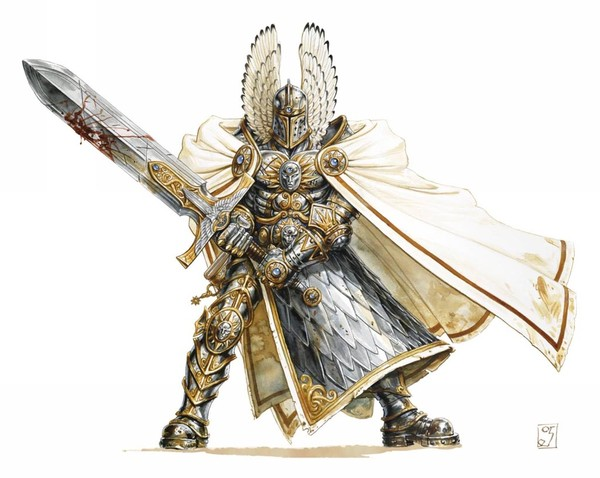
\includegraphics [width=40mm]{Images/Guerrier.jpg}\\
      
      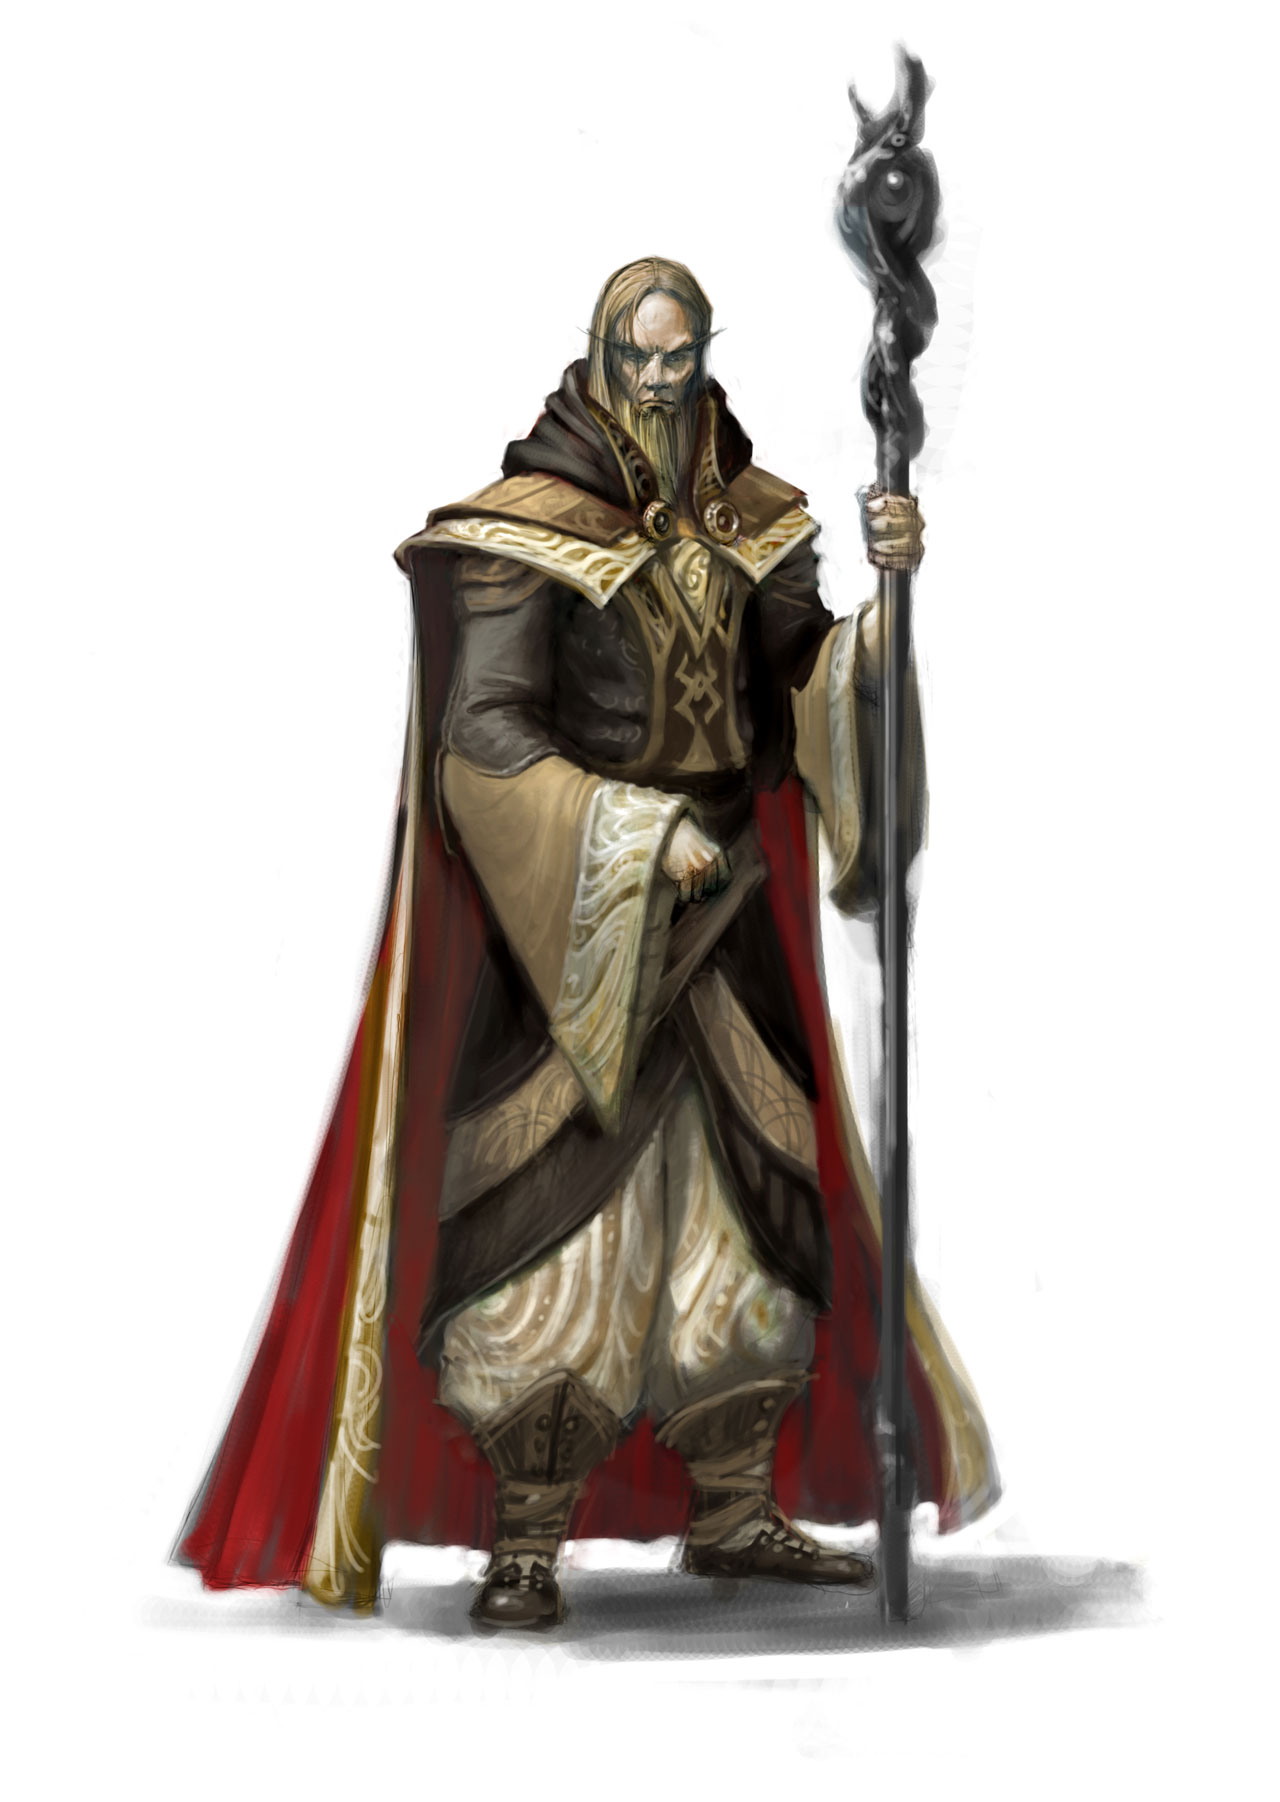
\includegraphics [width=40mm]{Images/Mage.jpg}& & 
\includegraphics [width=70mm]{Images/ENSEIRB-MATMECA.jpg} \\

      
      
      
    \end{tabular}
    
    
      
    \textsc{\Large \reportsubject}\\[0.5cm]
           {\large 01 fevrier 2012 - 31 juillet 2012}\\
           
           
           \HRule \\[0.4cm]
                  {\huge \bfseries \reporttitle}\\[0.4cm]
                  \HRule \\[1.5cm]
                  
                  \begin{center}
                    
                    \begin{flushleft} 
                      \large
                      \emph{Auteurs :}\\
                      
                      Arthur \textsc{HAVLICEK}, Louis \textsc{LE CLEC'H}\\ 
                      Sven \textsc{TATON}, Qiwen \textsc{LU}\\
                      
                    \end{flushleft}
                    
                    
                    \begin{flushright} 
                      \large
                      \emph{Responsables :} \\
                      M.~David \textsc{RENAULT - ENSEIRB-MATMECA} \\
                      M.~Yvan \textsc{LE BORGNE - LABRI}
                    \end{flushright}
                  \end{center}
                  
                  
                  %\vfill                  
                  
                  
                  
  \end{center}    
\end{center}
\end{titlepage}

  %\cleardoublepage % Dans le cas du recto verso, ajoute une page blanche si besoin
  \tableofcontents % Table des matières
  \listoffigures
 % \sloppy          % Justification moins stricte : des mots ne dépasseront pas des paragraphes
  %\cleardoublepage
  
  \chapter*{Introduction}
\addcontentsline{toc}{chapter}{Introduction}

Nethack est un jeu de type rogue-like sortit en 1987 et comme son nom l'indique, il est le résultat d'un travail collaboratif via internet. C'est un jeu assez complexe et qui comporte une haute dose d'aléatoire. Le but du projet était de proposer une modification du jeu dans le but de pouvoir transposer un problème mathématique au jeu et de tester la performance d'une solution sous la forme d'un bot.




  
  \chapter{Gestion du projet}

\section{outils de gestion utilisés}

Gérer un groupe de projet de sept personnes est évidemment assez complexe, nous avons donc utilisés plusieurs outils pour nous aidés. Après la séparation en deux groupes, certains outils ont été abandonnés car ils n'était plus très interessant.

\subsection{Gestionnaire de version}

Nous avons utilisé le gestionnaire de version git pour notre projet. Notre idée de base était d'avoir une branche stable et une branche de développement par module. Cette organisation s'est révelée peu efficace et nous sommes revenus à une utilisation plus proche de subversion, où tout le monde developpaient sur la même branche. 

\subsection{Gestion des ressources}

Lors de la première partie du projet, nous avons utilisé le logiciel planner pour faire un diagramme de gantt. Ce logiciel est assez interessant car il permet de mettre a jour le diagramme de manière très simple et il affiche les différentes informations (comme par exemple l'avancement d'une tache) de manière claire.
Cependant, nous avons un peu délaissé cet outils dans la deuxième partie du projet car, à quatre, il était aussi simple de se répartir les taches oralement.



  
  \section{Fonctionnement Géneral} 


\section{Utilisation/maintenance modes de jeu}

Le projet peut être extensible à plusieurs réductions possibles, différentes, du jeu initial. Afin de réduire le jeu à un sous-problème, des patchs peuvent être appliqués au sources. Ces patchs sont modulaires, peuvent être repris en totalité ou en partie selon le sous-problème abordé. Ils sont appliqués aux sources et permettent de bâtir, dans notre cas, le binaire du jeu où les monstres, les pièges et la faim sont désactivés.

Pour rajouter de nouveaux modes de jeu, on peut de la même façon collecter des patchs (dont une partie peut être partagée avec d'autres modes) et les appliquer aux sources du jeu avant de le compiler, de façon automatique via le script d'installation.



  \chapter{Modification du noyau}

Nous modifions le noyau de Nethack en fonction de nos besoins et de l'environnement (l'ensemble de règles) dans lequel on souhaite faire évoluer les bots. Pour cela, nous utilisons un système de patch que l'on applique avant la compilation du jeu. Voici la description des différents patch qui ont été crées.

\section{Le patch middleman}

Nethack n'a pas été conçu pour que des bots puissent y jouer. Nous avons donc du apporter des modification au noyau pour pouvoir y greffer des bots. Celle-ci sont installée via le patch middleman. Les principales modifications sont l'appel aux fonctions d'installation du module middle man, et les modifications du makefile permettant d'intégrer les modules modifiés au jeu.   

\section{Simplification de l'environnement de jeu}

Ces patchs désactivent certaines règles du jeu:
\begin{description}
\item[disable-hunger :] Ce patch supprime la faim dans le jeu.
\item[disable-locks :] Ce patch empeche que les portes du jeu soient fermées a clé.
\item[disable-monster :] Ce patch retire les monstre du jeu.
\item[disable object :] Ce patch retire les objet du jeu (par example les baignoires).
\item[disable-traps :] Ce patch retire les pièges du jeu.
\end{description}

Rassemblés, ces patchs permettent d'effectuer le mode de jeu de recherche de portes secrètes. Ces patchs peuvent être réutilisés, mais il peut être facile d'en créer un autre si l'on souhaite modifier différement le jeu.

Le mode de jeu que nous étudierons par la suite sera le suivant : le but du sous-problème étudié est de découvrir le maximum de portes cachées en un nombre fixé de tours (nous avons choisi 10000). Cet objectif d'exploration simule une situation du jeu initial où le joueur cherche à explorer de façon maximale le donjon dans un temps limité. Nous évaluerons donc les bots sur leur capacité à trouver efficacement des portes sur le maximum de niveaux.



  \chapter{Architecture}

  \section{Presentation de l'architecture}

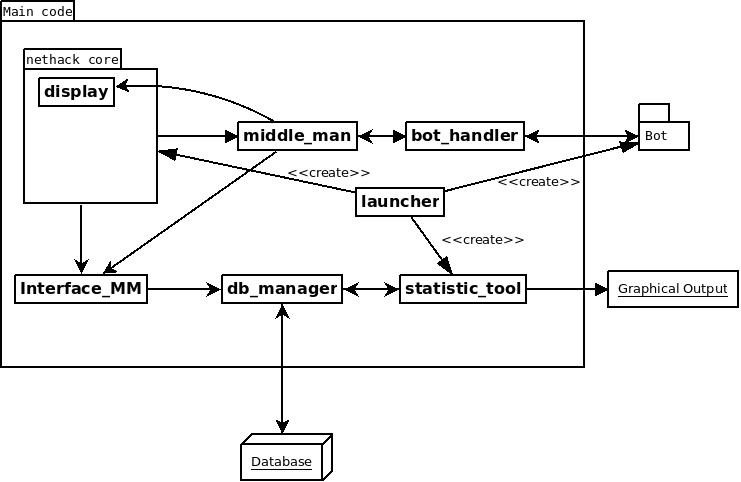
\includegraphics[width=140mm]{Images/new_archi.jpeg}

\begin{description}
\item[Bot Handler: ] Le Bot Handler est la pour traduire le langage haut niveau utilisé par le bot en commande Nethack.
\item[Middle Man: ] le Middle Man communique les instructions Nethack au noyau du jeu et et les messages du jeu au bot via le Bot Handler.
\item[Interface Middle Man: ] L'interface Middle Man transfert les statistiques et les caractéristiques d'une partie dans la base de donnée.
\item[DB Manager :] Le DB Manager est un module contenant les fonctions de manipulation de la base de donnée.
\item[Statistic Tools:] Ce module met en pages les informations contenues dans la base de donnée.  
\end{description}

  
  \section{Bot Handler}

%\paragraph{}
Le bot handler est l'ensemble de fonctions permettant assurant le dialogue
entre le bot et le noyau du jeu. Il s'agit d'un module C qui dépend uniquement de
l'interface fournie par le middle man.

%\paragraph{}
Le bot handler assure la traduction des entrées clavier comprises par nethack en 
leur équivalent en un langage plus lisible. Il balise et construit les messages destinés
au bot, et assure la traduction inverse des messages qu'il reçoit de la part du bot.

%\paragraph{}
Le bot handler attend la connexion d'un bot sur un port réseau, constant dans le module.
A chaque tour correspond l'envoi d'un message sur ce canal, puis une écoute de la réponse
correspondante. La réponse est traduite en entrée clavier nethack puis transmises au middle man.



  \section{Middle Man}
%\paragraph{}
Le middle man est un intermédiaire entre le noyau du jeu nethack
et les sources permettant le dialogue avec les bots. Il s'aagit d'un module C,
couplé d'un patch qui permet de l'installer dans le jeu.

%\paragraph{}
Dans le code de nethack,
il est installé comme une substitution aux événements qui sont relatifs
à l'interface utilisateur. Les fonctions du middle man sont appelé lorsque le
noyau attend une entrée clavier ou affiche un caractère sur le terminal texte.
De cette façon, il est impossible pour le bot de "tricher" : les informations 
collectées correspondent aux informations qu'un utilisateur peut lire à l'écran.

%\paragraph{}
Lorsqu'il intercepte une attente d'entrée clavier, le middle man active le
bot handler en lui fournissant la carte qu'il a créé au fur et à mesure des affichages.
Il attend de la part du bot qu'il effectue des actions. 

%\paragraph{}
Le middle man contient également d'autres points d'entrée permettant les collectes 
statistiques. Ces informations correspondent aux portes cachées dans le niveau, aux portes
ouvertes pendant la partie, aux portes secrètes totales, et à la plus grande
profondeur du donjon atteinte.

%\paragraph{}
Un nombre de tour maximal est fixé par une constante du module.
Après ce maximum, la partie est interrompue, et les statistiques sont transmises aux modules de
base de données.


  
  \chapter{Interface Middle Man} 


  \section{DB Manager} 

Le module DB MAnager est une simple interface permettant d'utiliser les fonction Fournie par le système de gestion de base de données SQLITE. Il s'agit d'une couche d'abstraction, permettant au besoin de changer de SGBD et donc d'augmenter la maintenabilité du code. 




  \include{k_Module_StatisticTools}

  \chapter{Bot}

Les bots sont completement indépendants du jeu. Cela signife qu'ils peuvent être écrits dans n'importe quel langage de programmation, les seuls prérequis étant de pouvoir ouvrir une socket et d'envoyer des chaînes de caractères.

\section{Développer un bot}

\subsection{Etablir la communication avec Nethack}
Le bot et Nethack communiquent via une socket de type internet dont le port est 4242. Ce port est écrit en dur dans le code.

\subsection{Envoyer des ordres}
Le bot doit utiliser un langage haut niveau pour communiquer ses ordres au jeu.

\begin{description}
\item[SEARCH :] permet de rechercher une porte secrète.
\item[OPEN :] permet d'ouvrir une porte.
\item[FORCE :] permet de forcer l'ouverture d'une porte.
\item[MOVE :] permet de se déplacer.
\item[DOWN :] permet de descendre des escalier. 
\item[UP :] permet de monter des escalier.
\end{description}

Certains ordres nécessitent d'être suivi d'une direction pour être exécutés. Ces directions ont également été traduites, elle correspondent aux points cardinaux en anglais et en majuscules (NORTH, SOUTH\_WEST etc). Nous avons également ajouté UP et DOWN, qui correspondent aux escaliers du donjon et permettent d'accéder aux niveaux supérieurs et inférieurs.

Le bot ne peut envoyer qu'un ordre par tour. Une fois celui-ci envoyé il faut donc se mettre a l'écoute du jeu qui va nous envoyer un certain nombre d'information (par exemple la carte du jeu). La liste des ordres peut-être modifiée via le Bot Handler.

\subsection{Information renvoyée par le jeu}
Lorsque le jeu reçoit un ordre, il l'applique, puis renvoie la carte mise à jour sous la forme d'une chaîne de caractère. Si l'on souhaite avoir un bot un peu évolué, il peut être interessant de la stocker. 

la chaine de caractère envoyée par le jeu a pour forme:

\begin{verbatim}
START
DUNGEON_LEVEL 1
MAP_HEIGHT 6
MAP_WIDTH 10
START MAP
          
   ----   
  |...@+  
  |....|  
   ----   
          
END MAP
END
\end{verbatim}



\section{Exemple d'un bot codé en java}

Nous avons codés deux bots relativement simple en java. L'un est completement aléatoire, l'autre est plus évolué. Nous allons ici décrire le fonctionnement du second.

\subsection{Diagramme de classe}

Voir l'annexe.
 
\subsection{Description}

Voici une description rapide de la plupart des classes du bot:

\begin{description}
\item[Map :] Cette classe permet de stocker et de manipuler la carte.
\item[Bot :] Cette classe permet de programmer le comportement du bot.
\item[InputOutputUnit :] Cette classe permet de gérer les connexions avec le Bot Handler.
\item[SquareType :] Cette classe contient tout les types de case pouvant être présent sur la carte.
\item[Protocole :] Cette classe contient les commandes à envoyer au Bot Handler.
\item[StepMap :] Contient certaines methodes permettant d'ameliorer l'algorithme du bot.
\item[Direction :] Cette classe contient des variables de directions.
\item[Variables :] Cette classe contient des variables diverses (comme ACTION\_RESULT par exemple).
\end{description} 

\subsection{Algorithme}

L'algorithme du bot est relativement simple, il se déplace de manière aléatoire sur la carte et garde en mémoire les cases déjà visitées. A chaque tour, le bot choisi une case parmi celle qu'il a le moins visité. 

\subsection{}


  \chapter*{Conclusion}
\addcontentsline{toc}{chapter}{Conclusion}


  
  \chapter*{Annexe}
\addcontentsline{toc}{chapter}{Annexe}



\end{onehalfspace}
\end{document}
